% !TeX spellcheck = hu_HU
\documentclass[12pt,a4paper]{article}
\usepackage[utf8]{inputenc}
\usepackage{cmap}
\usepackage[T1]{fontenc}
\usepackage[magyar]{babel}
\usepackage{amsmath}
\usepackage{amsfonts}
\usepackage{amssymb}
\usepackage{graphicx}

\usepackage{outlines}

\usepackage{hyperref}
\hypersetup{ colorlinks=true, linkcolor=blue }

\hyphenpenalty=10000

\begin{document}

\begin{center}
	\huge
	Valószínűségszámítás és statisztika\\
	\vspace{1mm}
	\LARGE
	Statisztika témakör jegyzet\\
	\vspace{5mm}
	\large
	Készült Zempléni András előadásai\\
	és Kovács Ágnes gyakorlatai alapján\\
	\vspace{5mm}
	Sárközi Gergő, 2021-22-2. félév\\
	Nincsen lektorálva!
\end{center}

\tableofcontents

\pagebreak

\section{Előadás 7: Statisztika bevezetés}

\begin{outline}
	\1 Két fő ág: leíró (újságokba), matematikai (becsléselmélet, hipotizéselmélet)
	\1 Lényeges, hogy válaszainkat értelmezzük, mondatban válaszoljunk: laikusuk is értsék meg az eredményt.
\end{outline}

\subsection{Leíró statisztika alapfogalmak}

\begin{outline}
	\1 Statisztikai egység: vizsgálat tárgyát képező egység
	\1 Statisztikai sokaság (populáció): egységek összessége, halmaza
		\2 Lehet hipotetikus is: gyár által jelenleg tervezett gyártandó termékek
	\1 Statisztikai adat: sokaságra vonatkozó számszerű jellemző, mérési eredmény
	\1 Statisztikai ismérv: sokaság egyedeit jellemző tulajdonság
	\1 Ismérvváltozatok: ismérvek lehetséges kimenetelei
	\1 Minta: sokaság véges számosságú részhalmaza
	\1 Statisztikai következtetés: teljes sokaságot nem ismerjük, de a minta alapján következtetünk valamit a teljes sokaságról
\end{outline}

\subsubsection{Ismérvek típusai}

\begin{outline}
	\1 Első kategória
		\2 Minőségi: számszerűen nem mérhető
		\2 Mennyiségi: számszerűen mérhető, lehet diszkrét vagy folytonos
		\2 Időbeli
		\2 Területi
	\1 Második kategória
		\2 Közös: sokaság egyedei között egyformák
		\2 Megkülönböztető: sokaság egyedei között eltérőek
\end{outline}

\pagebreak

\subsubsection{Mérési skálák (mérési szintek)}

\begin{outline}
	\1 Névleges (nominális): hozzárendelt számok csak megkülönböztetnek, műveleteket végezni rajtuk értelmetlen (pl. személy neme)
	\1 Sorrendi (ordinális): valamilyen tulajdonság alapján sorba rendezünk, egyedek tulajdonsága közötti különbséget nem tudjuk mérni (pl. érdemjegy)
	\1 Intervallumskála: skálaértekek különbségei is valós infót adnak, a nullpont meghatározása a skálán önkényes (pl. hőmérséklet C-ben)
	\1 Aranyskála: skálának van valódi nullpontja és minden matematikai művelet végezhető (pl. személyek magassága)
	\1 Metrikus skála (ritkán használt): intervallum és aranyskála közös neve
\end{outline}

\subsubsection{Statisztikai tábla}

\begin{outline}
	\1 Statisztikai sorok összefüggő rendszere
	\1 Egyszerű tábla: nincsenek csoportok, összegző sorok
	\1 Csoportosító tábla:
		\2 Egyetlen csoportosító szempont
		\2 Gyakoriság van csak benne: hányan esnek a csoportba
	\1 Kombinációs tábla, kontingenciatábla, kereszttábla:
		\2 Legalább két csoportosító szempont
		\2 Gyakoriságok vannak csak benne
\end{outline}

\pagebreak

\subsection{Statisztikai elemzés lépései}

\begin{outline}
	\1 Tervezés: mit vizsgálunk, hogyan gyűjtünk adatot, előzetes sejtések/hipotézis
	\1 Adatgyűjtés
	\1 Adatbevitel
	\1 Adatok validálása: nyilván rossz értékek kiszűrése (pl. negatív életkor)
	\1 Adatelemezés, adatellenőrzés (leíró statisztika, grafikonok)
	\1 Hibás adatok kijavítása vagy kihagyása
		\2 Lehetőleg ki kell javítani, nem pedig kidobni (nehéz feladat)
	\1 Adatelemzés, statisztikai következtetések levonása (matematikai statisztika)
	\1 Eredmények értelmezése, visszacsatolás
\end{outline}

\subsection{Mennyiségi sorok elemzése}

\begin{outline}
	\1 Ismérv diszkrét $\implies$ gyakorisági sort készítünk
	\1 Ismérv folytonos vagy sok van belőle: osztályközös gyakorisági sor
		\2 Összevonunk több ismérvet: $A_i$ és $B_i$ közötti gyakoriságot számolunk
	\1 Gyakori jelölések: $n$ a minta mérete, $k$ az ismérvértékek (sorok) száma, $f_i$ a gyakoriság és $x_i$ (vagy $x_{i,a} - x_{i,f}$ ha nem diszkrét) az ismérvérték
		\2 Osztályközös esetén $x_i$ az osztályközepet jelöli: $x_i = \frac{x_{i,a} + x_{i,f}}{2}$
\end{outline}

\subsection{Középértékek számolása}

\begin{outline}
	\1 Mintaátlag, közvetlen adatból: $\overline{x} = \frac{\sum_{i=1}^{n} x_i}{n}$
	\1 Mintaátlag, osztályközös gyakorisági sorokból: $\overline{x} = \frac{\sum_{i=1}^{n} f_i*x_i}{n}$
	\1 Módusz: legtöbbször előforduló ismérvérték
	\1 Medián: sorba rendezés után középső elem (rendezett minta: $X^*$)
		\2 $Me = \begin{cases}
		x^*[\frac{n+1}{2}] & \text{ ha $n$ páratlan}\\
		\frac{1}{2}*(x^*[\frac{n}{2}] + x^*[\frac{n}{2}+1]) & \text{ ha $n$ páros}
		\end{cases}$
\end{outline}

\pagebreak

\subsection{Kvantilisek}

\begin{outline}
	\1 y-kvantilis: $q_y = \inf\{ x \;|\; F(x) \ge y \}$
		\2 Ha $F$ invertálható: $q_y = F^{-1}(y)$
	\1 Tapasztalati $y$-kvanatilis: ismérvérték; mintaelemek $y$-ad része $\le$ nála
		\2 Sokféleképpen számolható, interpolációs módszer az egyik:
		\2 Sorszám megállapítása ($e$ egészrész, $t$ törtrész): $(n+1)y=e+t$
		\2 Kvantilis kiszámolása: $q_z = X^*_e + t(X^*_{e+1} - X^*_e)$
	\1 Jelölje $q_y$ a tapasztalati $y$-kvantilist
	\1 Tercilisek: $T_1 = q_{1/3}$, $T_2 = q_{2/3}$
	\1 Kvartilisek: $Q_1 = q_{1/4}$ (alsó), $Q_2 = Me = q_{2/4}$, $Q_3 = q_{3/4}$ (felső)
	\1 Percentilisek: $P_i = q_{i/100}$ ahol $i = 1,2,...,99$
\end{outline}

\subsection{Tapasztalati eloszlás}

\begin{outline}
	\1 Minden megfigyeléshez $\frac{1}{n}$ súlyt rendelünk $\implies$ diszkrét eloszlás
	\1 $\overline{X} = E(X)$
	\1 Tapasztalati eloszlásfüggvény: $F_n(x) = \frac{1}{n} * \sum_{i=1}^{n} I(x_i < x)$
		\2 $I$ az indikátor, értéke $0$ (ha $X_i < x$) vagy $1$ (ha $X_i \ge x$)
		\2 Ábrázolva: ahol szakadás van, azt az értéket tudja felvenni\\
		(az ugrás mértéke a valószínűség)
	\1 k-adik tapasztalati momentum: $m_k = \frac{1}{n} * \sum_{i=1}^n X_i^k$
	\1 Glivenko-Cantelli tétel: tapasztalati eloszlásfüggvény ($F_n(x)$) és az elméleti eloszlásfüggvény ($F(x)$) közötti eltérés maximuma 1 valószínűséggel 0-hoz konvergál
		\2 Következmény: $F_n(x)$ közelít $F(x)$-hez ($\forall x$ esetén) a minta növésével
		\2 Elég nagy mintával tetszőleges közelséget el lehet érni
\end{outline}

\pagebreak

\subsection{Szóródási mutatók számolása}

\begin{outline}
	\1 Terjedelem (range): $R = x_n^* - x_1^*$
	\1 Interkvartilis terjedelem: $IQR = Q_3 - Q_1$
	\1 Tapasztalati szórás:
		\2 Átlagtól való átlagos négyzetes eltérés négyzetgyöke
		\2 Közvetlenül: $S_n = \sqrt{\frac{1}{n}*\sum_{i=1}^{n} (x_i - \overline{x})^2}$
		\2 Osztályközös gyakoriságból: $S_n = \sqrt{\frac{1}{n}*\sum_{i=1}^{k} f_i (x_i - \overline{x})^2}$
	\1 Korrigált tapasztalati szórás:
		\2 Átlagtól való korrigált átlagos négyzetes eltérés négyzetgyöke
		\2 Ez az alapértelmezett általában
		\2 Számítás: ugyan az, csak $n$ helyett $n-1$-gyel osztunk (Jele: $S^*_n$)
		\2 Kis s-sel jelölés jelentése: nem a valószínűségi változóról, hanem a konkrét értékről van szó (nem nagyon számít, csak így helyesebb)
	\1 Szórási együttható, relatív szórás: $V=S_n/\overline{X}$ ($*100\%$)
\end{outline}

\pagebreak

\subsection{Grafikus megjelenítés}

\begin{outline}
	\1 Kördiagram rossz
\end{outline}

\subsubsection{Hisztogram}

\begin{outline}
	\1 Osztályok gyakoriságát ábrázolja ($y$ az $f_i$ gyakoriság, $x$ az ismérv)
	\1 Osztályok száma $k$, hosszuk (ha azonos): $h = \frac{x^*_n - x^*_1}{k}$
	\1 Sűrűséghisztogram: $g_i = \frac{f_i}{n*h_i}$
		\2 Relatív gyakoriság / intervallumhossz értéket ábrázoljuk
		\2 Területarányos, összterület=1
\end{outline}

\subsubsection{Boxplot ábra (Box \& Whiskers diagram)}

\begin{figure}[h!]
	\centering
	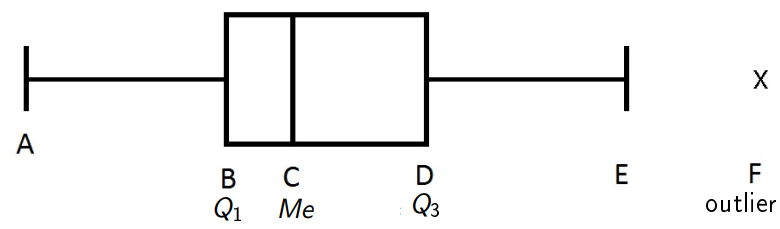
\includegraphics[width=0.7\linewidth]{boxplot}
\end{figure}

\begin{outline}
	\1 A = $max\{ x^*_1; Q_1 - 1.5 * IQR \}$
	\1 E = $min\{ x^*_n; Q_3 + 1.5 * IQR \}$
\end{outline}

\pagebreak

\section{Előadás 8: Matematikai statisztika, becsléselmélet}

\subsection{Matematikai statisztika}

\begin{outline}
	\1 Minta alapján teljes populáció tulajdonságaira következtetés
	\1 Paramétertér: $\Theta$ (1 vagy több dimenziós, akár végtelen) ($\vartheta \in \Theta$)
	\1 Minta: $X = (X_1, X_2, ..., X_n)$ i.i.d. valószínűségi változók sorozata
		\2 Minta realizációja ($x_1,...,x_n$): konkrét értékeket kap
	\1 Mintatér: $\mathcal{X} : \mathbb{R}^n$, ide eshetnek a mintaelemek
	\1 Mintaelemek eloszlása ($F$) ismeretlen, de paraméterezhető: $F_\vartheta$
	\1 Gyakori feladat: minta alapján adott eloszlás paraméterjének megállapítása
\end{outline}

\subsection{Becsléselmélet}

\subsubsection{Bevezetés, motiváció}

\begin{outline}
	\1 Legyen $X$ egy minta
	\1 Illeszkedésvizsgálat: milyen eloszlású lehet $X$?
	\1 Pontbecslés: ismert eloszlás esetén mi az eloszlás paramétere?
		\2 Mintából számoljuk, így valamennyi hiba van benne
		\2 A kapott eredményben nincs benne, hogy mennyire biztos a becslés
		\2 Példák erre: Maximum Likelihood, Momentum-módszer
	\1 Intervallumbecslés: milyen intervalban lesz nagy valószínűséggel $\vartheta$?
		\2 Csak egyetlen szám helyett egy intervallum az eredmény
		\2 Intervallum hosszából következtethető, hogy mennyi biztos a becslés
		\2 Példa erre: konfidenciaintervallum (következő EA)
\end{outline}

\pagebreak

\subsubsection{Alapdefiníciók}

\begin{outline}
	\1 Legyen $X = (X_1, ..., X_n)$ i.i.d. minta egy $\vartheta \in \mathbb{R}$ paraméterű eloszláscsaládból
	\1 $T : \mathcal{X} \to \mathbb{R}$ becslés $\vartheta$-ra
		\2 Torzítatlan $\Leftrightarrow$ $E_\vartheta(T(X)) = \vartheta$ \;\;\; ($\forall \vartheta \in \Theta$)
		\2 Aszimptotikusan torzítat $\Leftrightarrow$ $E_\vartheta(T_n(X)) \to \vartheta$ ha $n \to \infty$ ($\forall \vartheta \in \Theta$)
		\2 Konzisztens $\Leftrightarrow$ $T_n(X) \to \vartheta$ sztochasztikusan ha $n \to \infty$ ($\forall \vartheta \in \Theta$)
			\3 Elégséges, ha $T_n$ aszimptotikusan torzítatlan és $D^2(T_n) \to 0$
\end{outline}

\begin{figure}[h!]
	\centering
	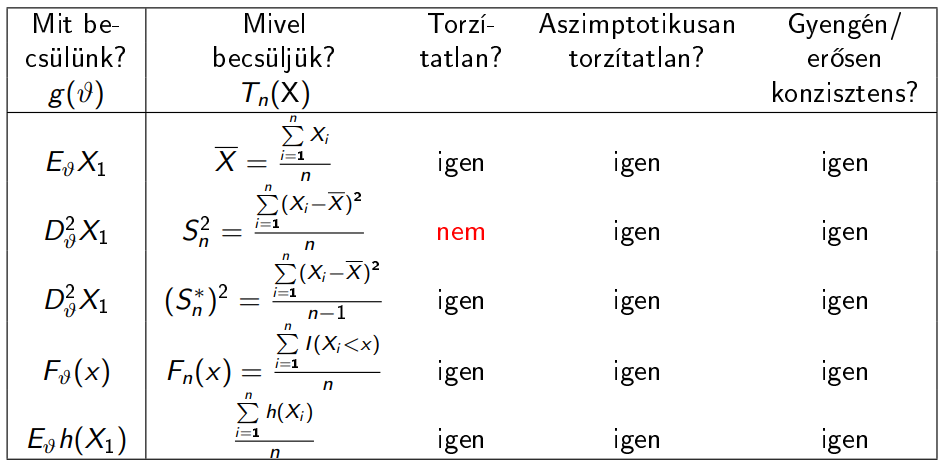
\includegraphics[width=1\linewidth]{becslések}
\end{figure}

\subsubsection{Likelihood függvények}

\begin{outline}
	\1 Likelihood függvény: $L(\vartheta;x)$
		\2 Folytonos eloszlás: $L(\vartheta;x) = f_\vartheta(x) = \Pi_{i=1}^n f_\vartheta(x_i)$
		\2 Diszkrét eloszlás:  $L(\vartheta;x) = P_\vartheta(X=x) = \Pi_{i=1}^n P_\vartheta(X_i = x_i)$
			\3 $\implies$ $x_i$ gyakorisága $g$, akkor $P_\vartheta(X_i = x_i)^g$-ként jelenik meg
	\1 Log-likelihood függvény (latex: ell): $\ell(\vartheta;x) = ln(L(\vartheta;x))$
	\1 $\sum_{i=1}^n x_i$ felírható $n * \overline{x}$ alakban (szebb)
	\1 $f_\vartheta(x)$-ban van elágazás és $x$ függ $\vartheta$-tól (pl. $0 \le x \le \vartheta$), akkor indikátor fv-t vegyünk be $f_\vartheta$-ba:
	$...*I(0 \le x_i \le \vartheta) \implies ... * I(0 \le x_1^*) * I(x_n^* \le \vartheta)$
		\2 Maximumot keresünk $\implies$ indikátor értéke legyen $1$
\end{outline}

\pagebreak

\subsection{Maximum likelihood becslés (ML-módszer) (pontbecslés)}

\begin{outline}
	\1 $L(\vartheta;x)$ maximumát keressük (ugyan ott van, mint $\ell(\vartheta;x)$ maximuma)
	\1 Maximum keresése deriválttal: $\partial_\vartheta \ell(\vartheta;x) = 0$
		\2 Nem szükséges további ellenőrzés: ahol $0$, ott a max
		\2 Több dimenziós $\vartheta$ esetén: $\partial_{\vartheta_i} \ell(\vartheta;x) = 0$
	\1 ML-becslés invariánsa: $\vartheta$ ML becslése $\hat{\vartheta}$ $\implies$ $g(\vartheta)$ ML-becslése $g(\hat{\vartheta})$
\end{outline}

\subsection{Nevezetes diszkrét eloszlások ML-becslése}

\begin{outline}
	\1 Egyes vizsgálatokhoz szükségünk lesz eloszlások paraméterének becslésére
	\1 Binomiális: $p = \frac{\overline{X}}{m} = \frac{0*db_1 + ... + m*db_m}{m * \sum_{i=1}^m db_i}$ ahol $m$ a másik paraméter
	\1 Poisson: $\lambda = \overline{X} = \frac{1}{n} * \sum_{i=1}^n k_i$
	ahol $k_i \ge 0$ az érték (nem gyakoriság)
	\1 Geometriai, Pascal: $\frac{1}{\overline{X}} = \frac{n}{\sum_{i=1}^n k_i}$
	ahol $k_i \ge 1$ az érték (nem gyakoriság)
	\1 Negatív binomiális, hipergeometriaia: nem találtam
\end{outline}

\subsection{Momentum módszer (pontbecslés)}

\begin{outline}
	\1 Tapasztalati és elméleti momentumokat egyenlővé tesszük
		\2 Tapasztalati momentum (mintából származik): $m_i = \frac{1}{n} \sum_{j=1}^{n} x_j^i$
		\2 Elméleti momentum: $M_i(\vartheta) = E_\vartheta(X^i)$
	\1 $i$ értékei: $1,...,p$ ahol $p$ a $\vartheta$ dimenzióinak száma (egyenletrendszer lesz)
		\2 Egy dimenziós $\vartheta$ esetén: $\overline{x} = m_1 = M_1 = E_\vartheta(X)$
		\2 Két dimhez segítség: $E(X^2) = D^2(X) + E^2(X)$ \; ($D^2(X)=...$-ból)
\end{outline}

\subsection{Becslés hibája, standard hiba}

\begin{outline}
	\1 Becslés standard hibája a becslés szórása
	\1 $s.e.(\overline{X}) = \frac{\sigma}{\sqrt{n}}$ \;\; (azaz 0-hoz tart, ahogy az elemszám nő)
	\1 $\sigma$ ismeretlen $\implies$ becsüljük:
	$\widehat{s.e.}(\overline{X}) = \frac{\widehat{\sigma}}{\sqrt{n}}$
		\2 Nem torzítatlan, csak aszimptotikusan
\end{outline}

\pagebreak

\subsection{Konfidenciaintervallum (intervallumbecslés)}

\begin{outline}
	\1 Intervallum, ami legalább $1 - \alpha$ valószínűséggel tartalmazza a paramétert minden $\vartheta$ értékre
		\2 Azaz a valódi $m$ vagy $\sigma$ ekkora valószínűséggel van az intervallumban
		\2 100 szimulációból kb. $(1-\alpha)*100$-szor lesz az intervallumban
	\1 Mi elsősorban normál eloszlással fogunk csak dolgozni
	\1 Emlékeztető: $\frac{\overline{X}-m}{\frac{\sigma}{\sqrt{n}}} \sim N(0;1)$
	\1 $u_x$ jelentése: $x$-hez tartozó $N(0;1)$ eloszlás kvantilis ($\Phi(u_x) = x$)
	\1 $t_x$ jelentése: $x$-hez tartozó $n-1$ szabadsági fokú $t$ eloszlás kvantilis
	\1 Intervallum hossza csökken, ha $n$ nő és ha $\sigma$ csökken
	\1 Intervallum hossző nő, ha $\alpha$ csökken
\end{outline}

\subsubsection{Kétoldali $1 - \alpha$ megbízhatóságú konfidenciaintervallum}

\begin{outline}
	\1 $m$-re, ha $\sigma$ ismert:
	$\overline{X} \pm u_{1-\frac{\alpha}{2}} * \frac{\sigma}{\sqrt{n}}$
		\2 \begin{verbatim}
			ci_also <- mean(sample) - qnorm(1 - alpha / 2) * sigma / sqrt(n)
			ci_felso <- mean(sample) + qnorm(1 - alpha / 2) * sigma / sqrt(n)\end{verbatim}
		\2 Szükséges elemszám adott intervallum hosszhoz: \begin{verbatim}
			hossz <- 8
			legalabbn <- (2 * qnorm(1 - alpha / 2) * sigma / hossz)^2
			\end{verbatim}
	\1 $m$-re, ha $\sigma$ ismeretlen:
	$\overline{X} \pm t_{n-1;1-\frac{\alpha}{2}} * \frac{S^*_n}{\sqrt{n}}$
		\2 \begin{verbatim}
			sd <- sd(sample)
			ci_also <- mean(sample) - qt(1 - alpha / 2, df=n-1) * sd / sqrt(n)
			ci_felso <- mean(sample) + qt(1 - alpha / 2, df=n-1) * sd / sqrt(n)\end{verbatim}
	\1 $\sigma^2$-re: $[ \frac{(n-1) * (S^*_n)^2}{\chi^2_{n-1;1-\frac{\alpha}{2}}}
	; \frac{(n-1) * (S^*_n)^2}{\chi^2_{n-1;\frac{\alpha}{2}}} ]$
\end{outline}

\pagebreak

\subsubsection{Egyoldali, alsó, $1 - \alpha$ megbízhatóságú konfidenciaintervallum}

\begin{outline}
	\1 $m$-re, ha $\sigma$ ismert:
	$(-\infty; \overline{X} + u_{1-\alpha} * \frac{\sigma}{\sqrt{n}})$
		\2 \begin{verbatim}
			ci_felso <- mean(sample) + qnorm(1 - alpha) * sigma / sqrt(n)\end{verbatim}
		\2 Szükséges elemszám adott intervallum hosszhoz: \begin{verbatim}
			hossz <- 8
			legalabbn <- (2 * qnorm(1 - alpha) * sigma / hossz)^2
			\end{verbatim}
	\1 $m$-re, ha $\sigma$ ismeretlen:
	$(-\infty; \overline{X} + t_{n-1;1-\alpha} * \frac{S^*_n}{\sqrt{n}})$
		\2 \begin{verbatim}
			sd <- sd(sample)
			ci_felso <- mean(sample) + qt(1 - alpha, df=n-1) * sd / sqrt(n)\end{verbatim}
	\1 $\sigma^2$-re: $(0; \frac{(n-1) * (S^*_n)^2}{\chi^2_{n-1;\alpha}})$
\end{outline}

\begin{figure}[h!]
	\centering
	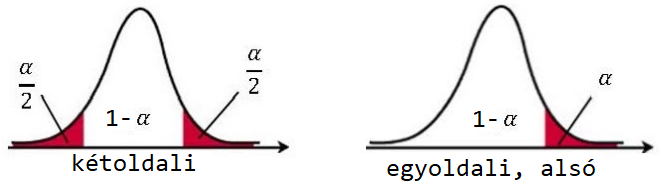
\includegraphics[width=0.5\linewidth]{konfidenciaintervallum}
\end{figure}

\pagebreak

\section{Előadás 9: Hipotézisvizsgálat, próbák}

\subsection{Hipotézisvizsgálat}

\begin{outline}
	\1 Hipotézis: állítás aminek igazságát vizsgálni szeretnénk: elfogadjuk/elutasítjuk
	\1 Paraméterteret diszjunkt részekre bontjuk: $\Theta = \Theta_0 \cup^* \Theta_1$
	\1 Nullhipotézis: $H_0 : \vartheta \in \Theta_0$\\
	Ellenhipotézis, alternatív hipotézis: $H_1 : \vartheta \in \Theta_1$
	\1 Nullhipotézist nem "elfogadjuk", hanem "nem tudjuk elvetni".\\
	Viszont elutasítani el tudjuk.
	\1 Nullhipotézis megválasztása: sok éves tapasztalatnak feleljen meg, reméljük teljesülését, aminek elutasítása negatív következménnyel jár (pl. bírság)
		\2 Az ellenhipotézis a lényeg, arról fogunk dönteni.
		\2 Egyenlőségjel mindig a nullhipotézisbe kerül.
	\1 Próba: segítségével döntés hozás a hipotézisről
		\2 Statisztikai próba vagy próba: minta alapján hozunk döntést
		\2 Paraméteres próba: eloszlás típusa ismert, a nullhipotézis az eloszlás paraméterére (vagy annak egy függvényére) vonatkozik
			\3 Továbbiakban ezzel fogunk általában foglalkozni
			\3 Továbbiakban legyen $\Theta \subset \mathbb{R}$, azaz a paraméter valós
	\1 Mintateret diszjunkt részekre bontjuk: $\chi = \chi_e \cup^* \chi_k$
		\2 $\chi_k$, kritikus tartomány: megfigyelések, amikre elutasítjuk $H_0$-t
		\2 $\chi_e$, elfogadási tartomány: megfigyelések, amikre elfogadjuk $H_0$-t
	\1 Döntési mátrix hipotézisvizsgálat esetén:
\end{outline}

\begin{table}[h]
	\centering
	\begin{tabular}{|c|c|c|}
		\hline
		$\downarrow$ valóság | döntés $\to$ & elfogadjuk ($\chi_e$) & elutasítjuk ($\chi_k$) \\
		\hline
		$H_0$ teljesül ($\Theta_0$) & helyes döntés & elsőfajú hiba \\
		\hline
		$H_0$ nem teljesül ($\Theta_1$) & másodfajú hiba & helyes döntés \\
		\hline
	\end{tabular}
\end{table}

\pagebreak

\subsection{Hiba valószínűségek, erőfüggvény, terjedelem}

\begin{outline}
	\1 Elsőfajú hiba valószínűsége:
		\2 Egyszerű $H_0$, $|\Theta_0| = 1$:
		$\alpha(\vartheta) = P_\vartheta(X \in \chi_k) = P_0(\chi_k)$
		\;\; ($\vartheta \in \Theta_0$)
		\2 Összetett $H_0$, $|\Theta_0| > 1$:
		$\alpha \ge P_\vartheta(X \in \chi_k)$ \;\; ($\forall \vartheta \in \Theta_0$)
	\1 Másodfajú hiba valószínűsége:
	\\$\beta(\vartheta) = P_\vartheta(X \in \chi_e) = P_1(\chi_e)
		= 1 - P_\vartheta(\chi_k)$ \;\; ($\vartheta \in \Theta_1$)
	\1 Erőfüggvény: $\psi(\vartheta) = 1 - P_\vartheta(\chi_e) = P_\vartheta(\chi_k)$
	ahol $\vartheta \in \Theta_1$
		\2 Jelentése: valószínűsége $H_0$ elvetésének, amikor az hamis
		\2 Valószínűsége annak, hogy egy adott különbséget egy adott mintanagyság és terjedelem mellett ki egy statisztikai próba kimutat
	\1 Terjedelem, pontos terjedelem, szignifikanciaszint: $\alpha = \sup_{\vartheta \in \Theta_0} \alpha(\vartheta)$
		\2 Általában feladat elejekor 5\%-on (vagy 1\% és 10\% között) rögzített
		\2 Megbízhatósági szint, konfidenciaszint: $1 - \alpha$ \; ($*100\%$)
			\3 Valószínűsége, hogy $H_0$-t elfogadjuk, amikor az igaz
		\2 Másképp: elsőfajú hiba valószínűsége $\alpha$ lesz
\end{outline}

\subsection{Próbák bevezetés}

\begin{outline}
	\1 Kétoldali próba: $H_0: \vartheta = \vartheta_0$ és $H_1: \vartheta \ne \vartheta_0$
	\1 Egyoldali próba: $H_0: \vartheta = \vartheta_0$ és $H_1: \vartheta < \vartheta_0$ (vagy >)
	\1 Próbastatisztika: alkalmas T statisztika, amivel a $\chi_k$-t meghatározzuk
		\2 Kétoldali próbához: $\chi_k = \{ x \in \chi \;:\; |T(X)| > c \}$
		\2 Egyoldali próbához: $\chi_k = \{ x \in \chi \;:\; T(X) \lessgtr c \}$
		\2 $c$ neve: kritikus érték
			\3 Jellemzően függ a próba terjedelmétől $\implies$ $c_\alpha$-val jelöljük
			\3 $c_\alpha$ jelölés jelentése: $c_\alpha$ a $T(X)$ val. változó $\alpha$-kvantilise
		\2 Próba meghatározása: előre rögzített $\alpha$ terjedelemhez keressük azt a $c_\alpha$ értéket, amire a próba pontos terjedelme éppen $\alpha$
			\3 $\sup_{\vartheta \in \Theta_0} P_\vartheta(T(X) > c_\alpha) = \alpha$
\end{outline}

\pagebreak

\subsection{Hipotézisvizsgálat menete}

\begin{outline}
	\1 Terjedelem ($\alpha$) lefixálása, általában 5\%-on (megbízhatóság: $1 - \alpha$)
	\1 Nullhipotézis: sokévi tapasztalatnak megfelelő paramétertartomány
		\2 Az egyenlőség (pl. $\le$) mindig ide kerül
	\1 Alternatív hipotézis: feladat kérdéséhez megfelelő paramétertartomány
		\2 Erről be tudjuk látni, hogy igaz ($H_0$-ról csak "nem tudjuk elvetni")
		\2 Ezért a cél $H_1$ igazolása, azaz $H_0$ elvetése
	\1 Problémához alkalmas próba/próbák választása (egy/két oldali, stb.)
	\1 Próbastatisztika kiszámítása
\end{outline}

\subsubsection{Döntés minta és tartományok alapján}

\begin{outline}
	\1 Kritikus érték kiszámítása, kritikus tartomány megállapítása
		\2 Számolása általában: eloszlás kvantilis függvény "meghívása" $\alpha$-ra
	\1 $x \in \chi_k \;\;\Leftrightarrow\;\; H_1\text{-et elfogadjuk}$
	\1 Probléma: nem derül ki, hogy mennyire voltunk közel az elfogadáshoz
\end{outline}

\subsubsection{Döntés p-érték segítségével}

\begin{outline}
	\1 p-érték kiszámolása (számítógépes számolás esetén lehetőség)
		\2 Számolása általában: eloszlásfüggvény "meghívása" próbastatisztikával
		\2 Kétoldali próba esetén bonyolultabb (általában: $2*pDist(-|T|)$)
	\1 $p\text{-érték} < \alpha \;\;\Leftrightarrow\;\; x \in \chi_k
	\;\;\Leftrightarrow\;\; H_1\text{-et elfogadjuk}$
	\1 p-érték jelentése: terjedelem, amire a kritikus érték megegyezik a próbastatisztikával
		\2 Máshogy: legkisebb $\alpha$, amire az adott minta esetén elvetjük $H_0$-t
		\2 Máshogy: igaz $H_0$ mellett annak a valószínűsége, hogy a tapasztalt eltérést, vagy annál nagyobb eltérést kapunk
\end{outline}

\subsubsection{Elsőfajú, másodfajú hiba csökkentése}

\begin{outline}
	\1 $\alpha$ csökkentése $\beta$ növekedésével jár (ha minden más marad)
	\1 Mindkét hiba valószínűségének csökkentése: mintaelemszám növelése
\end{outline}

\pagebreak

\section{Előadás 10: Próbák normális eloszlás paramétereire}

\subsection{Használt jelölések, emlékeztetők}

\begin{outline}
	\1 Emlékeztető: $\frac{\overline{X}-m}{\frac{\sigma}{\sqrt{n}}}
	= \sqrt{n} * \frac{\overline{X}-m}{\sigma} \sim N(0;1)$
	\1 $u_x$ jelentése: $x$-hez tartozó $N(0;1)$ eloszlás kvantilis ($\Phi(u_x) = x$)
	\1 $t_x$ jelentése: $x$-hez tartozó $n-1$ szabadsági fokú $t$ eloszlás kvantilis
	\1 $S^*_n$ jelentése: korrigált tapasztalati szórás, $S^*_n = \sqrt{\frac{1}{n-1}*\sum_{i=1}^{n} (x_i - \overline{x})^2}$
\end{outline}

\subsection{Próbákról tudnivalók}

\begin{outline}
	\1 Kétmintás próba: két (összefüggő vagy független) mintánk van
	\1 Összefüggő (párosított) minták: vettünk egy mintát, valami megváltozott
	(pl. gépen valamit állítottunk) és veszünk még egy mintát ugyan onnan
		\2 Cél: változtatás hatásának vizsgálata (pl. működik-e a gyógyszer)
	\1 Kétoldali próba: egyenlőséget ellenőrzünk (pl. $m$ tényleg az-e)
	\1 Egyoldali próba: gyanúnk, hogy pl. $m$ valaminél kisebb/nagyobb
\end{outline}

\pagebreak

\subsection{Próbák normális eloszlás várható értékére ($m$)}

\begin{outline}
	\1 Egymintás próba
		\2 Szórás ismert: \hyperref[sec:próba-1minta-u]{egymintás u-próba}
		\2 Szórás ismeretlen: \hyperref[sec:próba-1minta-t]{egymintás t-próba}
	\1 Kétmintás próba, két minta független
		\2 Szórások ismertek: \hyperref[sec:próba-2minta-u]{kétmintás u-próba}
		\2 Szórások ismeretlenek: előzetes \hyperref[sec:próba-F]{F-próba} szükséges
			\3 Szórások megegyeznek: \hyperref[sec:próba-2minta-t]{kétmintás t-próba}
			\3 Szórások eltérnek: \hyperref[sec:próba-welch]{Welch-próba}
	\1 Kétmintás próba, két minta párosított (összefüggő)
		\2 Szórások ismertek: \hyperref[sec:próba-1minta-u]{egymintás u-próba} a különbségekre
		\2 Szórások ismeretlenek: \hyperref[sec:próba-1minta-t]{egymintás t-próba} a különbségekre
\end{outline}

\begin{figure}[h!]
	\centering
	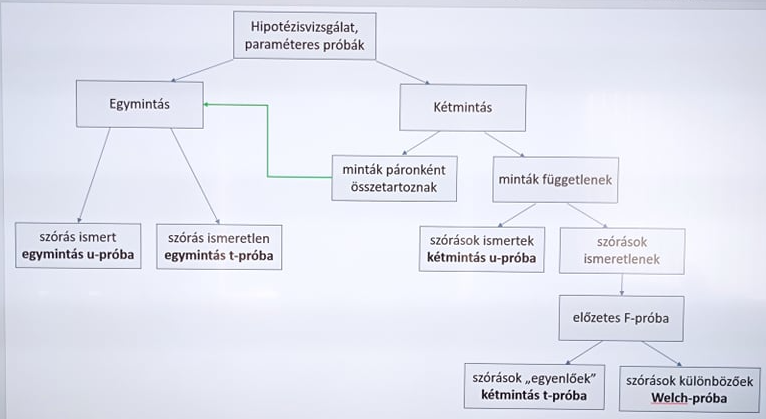
\includegraphics[width=1\linewidth]{paraméteres-próba-választás}
\end{figure}

\pagebreak

\subsubsection{Egymintás u-próba (z-test)}
\label{sec:próba-1minta-u}

\begin{outline}
	\1 $X_1,...,X_n \sim N(m,\sigma^2)$ ahol $\sigma$ ismert és $m=?$
	\1 Próbastatisztika: $T(X) = u = \sqrt{n}*\frac{\overline{X} - m_0}{\sigma}$
	\;\; ($H_0$ esetén $u \sim N(0,1)$)
		\2 \texttt{u <- sqrt(n) * (mean(sample) - mu0) / sigma}
	\1 Kétoldali: $H_0: m = m_0$ és $H_1: m \ne m_0$
	és $\chi_k = \{ x \;:\; |u| > u_{1-\alpha/2} \}$
		\2 \texttt{pertek <- 2*pnorm(-abs(u))}
		\2 \texttt{krit <- qnorm(c(alpha/2, 1-alpha/2)) \#1.alatt és 2.felett}
	\1 Egyoldali: $H_0: m = m_0$ és
		\2 $H_1: m < m_0$ és $\chi_k = \{ x \;:\; u < u_{\alpha} \}$
			\3 \texttt{pertek <- pnorm(u)}
			\3 \texttt{krit <- qnorm(alpha)}
		\2 $H_1: m > m_0$ és $\chi_k = \{ x \;:\; u > u_{1-\alpha} \}$
			\3 \texttt{pertek <- pnorm(-u)}
			\3 \texttt{krit <- qnorm(1-alpha)}
	\1 Kapcsolat konfidenciaintervallummal:
		\2 $|u| > u_{1-\alpha/2} \;\;\Leftrightarrow\;\; m_0 \notin
		(\overline{X} - u_{1-\alpha/2}*\frac{\sigma}{\sqrt{n}},\;\;
		\overline{X} + u_{1-\alpha/2}*\frac{\sigma}{\sqrt{n}})$
		\2 Máshogy: $H_0$-t pontosan akkor utasítjuk el, ha az $1-\alpha$ konfidenciaintervallum nem tartalmazza $m_0$-t
	\1 \begin{verbatim}
	library(TeachingDemos)
	z.test(x, alternative = c("two.sided/less/greater"),
	       mu = mu0, stdev = sigma, conf.level = 1 - alpha)
	\end{verbatim}
\end{outline}

\begin{figure}[h!]
	\centering
	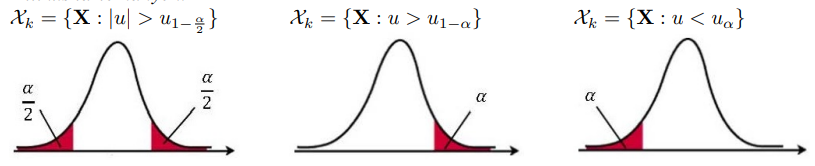
\includegraphics[width=1\linewidth]{kritikus-tartományok}
\end{figure}

\pagebreak

\subsubsection{Egymintás t-próba (Student's t-test)}
\label{sec:próba-1minta-t}

\begin{outline}
	\1 $X_1,...,X_n \sim N(m,\sigma^2)$ ahol $\sigma$ és $m$ ismeretlen; $m=?$
	\1 Próbastatisztika: $T(X) = t = \sqrt{n}*\frac{\overline{X} - m_0}{S^*_n}$
	\;\; ($H_0$ esetén $t \sim t_{n-1}$)
		\2 \texttt{t <- sqrt(n) * (mean(sample) - mu0) / sd(sample)}
	\1 Kétoldali: $H_0: m = m_0$ és $H_1: m \ne m_0$
	és $\chi_k = \{ x \;:\; |t| > t_{n-1,1-\alpha/2} \}$
		\2 \texttt{pertek <- 2*pt(-abs(t), df=n-1)}
		\2 \texttt{krit <- qt(c(alpha/2, 1-alpha/2), df=n-1) \#1.alatt és 2.felett}
	\1 Egyoldali: $H_0: m = m_0$ és 
		\2 $H_1: m < m_0$ és $\chi_k = \{ x \;:\; t < t_{n-1,\alpha} \}$
			\3 \texttt{pertek <- pt(t, df=n-1)}
			\3 \texttt{krit <- qt(alpha, df=n-1)}
		\2 $H_1: m > m_0$ és $\chi_k = \{ x \;:\; t > t_{n-1,1-\alpha} \}$
			\3 \texttt{pertek <- pt(-t, df=n-1)}
			\3 \texttt{krit <- qt(1-alpha, df=n-1)}
	\1 \begin{verbatim}
	t.test(x, alternative = "two.sided/less/greater",
	       mu = mu0, conf.level = 1 - alpha)
	\end{verbatim}
\end{outline}

\pagebreak

\subsubsection{Kétmintás u-próba}
\label{sec:próba-2minta-u}

\begin{outline}
	\1 Független minták: $X_{1..n} \sim N(m_1, \sigma_1^2)$ és $Y_{1..m} \sim N(m_2, \sigma_2^2)$
		\2 $\sigma_1$, $\sigma_2$ ismert és $m_1$, $m_2$ ismeretlen (relációjuk a kérdés)
	\1 Próbastatisztika: $T(X,Y) = u = (\overline{X} - \overline{Y}) / \sqrt{\frac{\sigma_1^2}{n} + \frac{\sigma_2^2}{m}}$
		\2 $H_0$ esetén $u \sim N(0,1)$
		\2 \begin{verbatim}
		u <- (mean(sampleA) - mean(sampleB))
		      / sqrt(sigmaA^2/n + sigmaB^2/m)
		\end{verbatim}
	\1 Kétoldali: $H_0: m_1 = m_2$; $H_1: m_1 \ne m_2$
	és $\chi_k = \{ (x,y) : |u| > u_{1-\alpha/2} \}$
		\2 \texttt{pertek <- 2*pnorm(-abs(u))}
		\2 \texttt{krit <- qnorm(c(alpha/2, 1-alpha/2)) \#1.alatt és 2.felett}
	\1 Egyoldali: $H_0: m_1 = m_2$ és 
		\2 $H_1: m_1 < m_2$ és $\chi_k = \{ (x,y) \;:\; u < u_{\alpha} \}$
			\3 \texttt{pertek <- pnorm(u)}
			\3 \texttt{krit <- qnorm(alpha)}
		\2 $H_1: m_1 > m_2$ és $\chi_k = \{ (x,y) \;:\; u > u_{1-\alpha} \}$
			\3 \texttt{pertek <- pnorm(-u)}
			\3 \texttt{krit <- qnorm(1-alpha)}
	\1 \begin{verbatim}
	two_sample_u_test <- function(sampleA, sampleB, sigmaA, sigmaB,
	                              alternative, conf_level) {
	  alpha <- 1 - conf_level; n <- length(sampleA); m <- length(sampleB)
	  u <- (mean(sampleA) - mean(sampleB)) / sqrt(sigmaA^2 / n + sigmaB^2 / m)
	  if (alternative == "t" || alternative == "two.sided") {
	    krit <- qnorm(c(alpha/2, 1 - alpha/2)); pertek <- 2 * pnorm(-abs(u))
	  } else if (alternative == "l" || alternative == "less") {
	    krit <- qnorm(alpha); pertek <- pnorm(u)
	  } else if (alternative == "g" || alternative == "greater") {
	    krit <- qnorm(1 - alpha); pertek <- pnorm(-u)
	  } else { cat("Invalid alternative: " + alternative); return() }
	  cat("Próbastatisztika:", u,
	      "\nKritikus tartomány:", krit[1], "alatt és", krit[2], "felett",
	      "\nP-érték:", pertek, "\nDöntés:", if (pertek < alpha)
	         { "H0 elutasítva" } else { "H0-t nem sikerült elvetni" }, "\n")
	} %sampleA, sampleB sorrendje: lásd jegyzet PDF, kétmintás t-próba
	\end{verbatim}
\end{outline}

\pagebreak

\subsubsection{Kétmintás t-próba}
\label{sec:próba-2minta-t}

\begin{outline}
	\1 Független minták: $X_{1..n} \sim N(m_1, \sigma_1^2)$ és $Y_{1..m} \sim N(m_2, \sigma_2^2)$
		\2 $\sigma_1 = \sigma_2$ ismeretlen és $m_1$, $m_2$ ismeretlen (relációjuk a kérdés)
	\1 Próbastatisztika: $T(X,Y) = t = \sqrt{\frac{n*m}{n+m}} * (\overline{X} - \overline{Y}) / \sqrt{\frac{(n-1)(S^*_1)^2+(m-1)(S^*_2)^2}{n+m-2}}$
		\2 $H_0$ esetén $t \sim t_{n+m-2}$
		\2 \begin{verbatim}
		t <- sqrt((n*m)/(n+m)) * (mean(sampleA) - mean(sampleB))
		/ sqrt( ((n-1)*sd(sampleA)^2 + (m-1)*sd(sampleB)^2) / (n+m-2) )
		\end{verbatim}
	\1 Kétoldali: $H_0: m_1 = m_2$ és $H_1: m_1 \ne m_2$\\
	és $\chi_k = \{ (x,y) : |t| > t_{n+m-2,1-\alpha/2} \}$
	\1 Egyoldali: $H_0: m_1 = m_2$ és 
		\2 $H_1: m_1 < m_2$ és $\chi_k = \{ (x,y) \;:\; t < t_{n+m-2,\alpha} \}$
			\3 \texttt{pertek <- pt(t)}
			\3 \texttt{krit <- qt(alpha)}
		\2 $H_1: m_1 > m_2$ és $\chi_k = \{ (x,y) \;:\; t > t_{n+m-2,1-\alpha} \}$
			\3 \texttt{pertek <- pt(-t)}
			\3 \texttt{krit <- qt(1-alpha)}
	\1 \begin{verbatim}
	t.test(sampleA, sampleB, alternative="two.sided/less/greater",
	       paired=FALSE, var.equal=TRUE)
	\end{verbatim}
		\2 A minta sorrend és a reláció egyezzen meg az ellenhipotézissel
		\2 Ez a kettő ekvivalens: sampleA,sampleB,less $\Leftrightarrow$ sampleB,sampleA,greater
\end{outline}

\pagebreak

\subsubsection{Welch-próba}
\label{sec:próba-welch}

\begin{outline}
	\1 Független minták: $X_{1..n} \sim N(m_1, \sigma_1^2)$ és $Y_{1..m} \sim N(m_2, \sigma_2^2)$
		\2 $\sigma_1 \ne \sigma_2$ ismeretlen és $m_1$, $m_2$ ismeretlen (relációjuk a kérdés)
	\1 Próbastatisztika: $T(X,Y) = t' = (\overline{X} - \overline{Y}) / \sqrt{\frac{(S^*_1)^2}{n}+\frac{(S^*_2)^2}{m}}$
		\2 $H_0$ esetén $t' \sim t_f$
		ahol $\frac{1}{f} = \frac{c^2}{n-1} + \frac{(1-c)^2}{m-1}$
		\2 $S^*_1 > S^*_2$ (így válasszuk) $\implies
		c = (\frac{(S^*_1)^2}{n}) / ( \frac{(S^*_1)^2}{n} + \frac{(S^*_2)^2}{m} )$
	\1 Kétoldali: $H_0: m_1 = m_2$ és $H_1: m_1 \ne m_2$\\
	és $\chi_k = \{ (x,y) : |t'| > t_{f,\alpha/2} \}$
	\1 Egyoldali: $H_0: m_1 = m_2$ és 
		\2 $H_1: m_1 < m_2$ és $\chi_k = \{ (x,y) \;:\; t < -t_{f,\alpha} \}$
		\2 $H_1: m_1 > m_2$ és $\chi_k = \{ (x,y) \;:\; t > t_{f,\alpha} \}$
	\1 \begin{verbatim}
	t.test(sampleA, sampleB, alternative="two.sided/less/greater",
	       paired=FALSE, var.equal=FALSE)
	\end{verbatim}
		\2 Két minta (sampleA, sampleB) sorrendje: lásd kétmintás t-próba
\end{outline}

\pagebreak

\subsection{Próbák normális eloszlás szórásnégyzetére ($\sigma^2$)}

\begin{outline}
	\1 Gyakorlaton nem foglalkozunk ilyennel, kivéve az (előzetes) F-próba
	\1 Egymintás próba: \hyperref[sec:próba-chi2]{$\chi^2$-próba}
	\1 Kétmintás próba: \hyperref[sec:próba-F]{F-próba}
\end{outline}

\subsubsection{F-próba}
\label{sec:próba-F}

\begin{outline}
	\1 Független minták: $X_{1..n} \sim N(m_1, \sigma_1^2)$ és $Y_{1..m} \sim N(m_2, \sigma_2^2)$
		\2 $m_1$, $m_2$ ismeretlen és $\sigma_1$, $\sigma_2$ ismeretlen (relációjuk a kérdés)
	\1 Próbastatisztika: $T(X,Y) = F = \frac{(S^*_2)^2}{(S^*_1)^2}$ \; ha $S^*_1 < S^*_2$
		\2 $H_0$ esetén $F \sim F_{n-1,m-1}$
	\1 Kétoldali: $H_0: \sigma_1 = \sigma_2$ és $H_1: \sigma_1 \ne \sigma_2$
		\2 vagy $\chi_k = \{ (x,y) : F < F_{n-1,m-1,\alpha/2} \}$
		\2 vagy $\chi_k = \{ (x,y) : F > F_{n-1,m-1,1-\alpha/2} \}$
		\2 Attól függ, hogy $S_1^*$ vagy $S_2^*$ a nagyobb
	\1 Egyoldali: $H_0: \sigma_1 = \sigma_2$ és 
		\2 $H_1: \sigma_1 < \sigma_2$ és $\chi_k = \{ (x,y) \;:\; F < F_{n-1,m-1,\alpha} \}$
		\2 $H_1: \sigma_1 > \sigma_2$ és $\chi_k = \{ (x,y) \;:\; F > F_{n-1,m-1,1-\alpha} \}$
	\1 Előzetes F-próba:
		\2 Mindig kétoldali
		\2 Nem számít a minták sorrendje (p-érték nem változik)
		\2 p-érték nagy $\implies$ nincs bizonyíték, hogy különböznek a szórások
			\3 Ha nem tudunk dönteni, inkább tekintsük a szórásokat egyenlőnek
		\2 \texttt{var.test(mintaA, mintaB, alternative="two.sided")}
		\2 \begin{verbatim}
		f <- sd(mintaA)^2 / sd(mintaB)^2
		pertek <- 2 * pf(f, df1 = length(mintaA) - 1,
		                    df2 = length(mintaB) - 1)
		\end{verbatim}
\end{outline}

\pagebreak

\subsubsection{$\chi^2$-próba}
\label{sec:próba-chi2}

\begin{outline}
	\1 $X_1,...,X_n \sim N(m,\sigma^2)$ ahol $\sigma$ és $m$ ismeretlen; $\sigma=?$
	\1 Próbastatisztika: $T(X) = h = \frac{(n-1)(S^*_n)^2}{\sigma_0^2}$
	\;\; ($H_0$ esetén $h \sim \chi^2_{n-1}$)
	\1 Kétoldali: $H_0: \sigma = \sigma_0$ és $H_1: \sigma \ne \sigma_0$
		\2 vagy $\chi_k = \{ x \;:\; h < \chi^2_{n-1,\alpha/2} \}$
		\2 vagy $\chi_k = \{ x \;:\; h > \chi^2_{n-1,1-\alpha/2} \}$
		\2 Attól függ, hogy $S_1^*$ vagy $S_2^*$ a nagyobb
	\1 Egyoldali: $H_0: m = m_0$ és 
		\2 $H_1: \sigma < \sigma_0$ és $\chi_k = \{ x \;:\; h < \chi^2_{n-1,\alpha} \}$
		\2 $H_1: \sigma > \sigma_0$ és $\chi_k = \{ x \;:\; h > \chi^2_{n-1,1-\alpha} \}$
	\1 Nem tételezünk fel normális eloszlást (a mintáról)
	\1 TODO teljes eseményrendszerről a dolgok
	\1 Alkalmazások: TODO
	\1 Nincs minden osztályban elég mennyiség: R adhat warning-ot
		\2 Ökölszabály: min. 5db minden osztályban ($n*p$ szorzás után)
		\2 Ha nincs elég, akkor vonjunk össze osztályokat:
			\3 \begin{verbatim}
			chisq.test(c(gyakorisag[1:3], sum(gyakorisag[4:5])),
			    p = c(p[1:3], sum(p[4:5]))) #utolsó 2 összevonva\end{verbatim}
			\3 \begin{verbatim}
			tbl2 <- cbind(tbl1[,"Left"] + tbl1[,"Neither"], tbl1[,"Right"])
			colnames(tbl2) <- c("Left+Neither", "Right")\end{verbatim}
\end{outline}

\pagebreak

\section{Előadás 11: illeszkedés-, homogenitás- és\\
függetlenségvizsgálat; regresszióelemzés}

\subsection{Diszkrét illeszkedésvizsgálat ($\chi^2$-próba)}

\begin{outline}
	\1 $H_0$: minta egy adott eloszlásból származik (valószínűségek egyeznek)
	\1 $H_1$: minta nem ilyen eloszlású (min 1x: várt, tap. valószínűségek $\ne$)
	\2 Próbastat.: $T_n(X) = \sum_{i=1}^{r} \frac{(N_i - np_i)^2}{np_i} \to \chi^2_{r-1}$
	(ha $H_0$ és $n \to \infty$)
	\2 Kritikus tartomány: $\chi_k = \{ x \;|\; T_n(x) > \chi^2_{r-1,1-\alpha} \}$
	\1 Tiszta illeszkedésvizsgálat: feltételezett eloszlás ismert
	\1 Becsléses illeszkedésvizsgálat: eloszlás paramétere ismeretlen
		\2 ML-módszerrel $s$ darab paramétert meg kell becsülni
		\2 Próbastatisztika ekkor $H_0$ esetén $\chi^2_{r-1-s}$-be tart
\end{outline}

\begin{table}[h]
	\centering
	\begin{tabular}{|c|c|c|c|c|}
		\hline
		Osztály & 1 & ... & r & Összesen \\
		\hline
		Gyakoriság & $v_1$ & ... & $v_r$ & n \\
		\hline
		Valószínűség & $p_1$ & ... & $p_r$ & 1 \\
		\hline
	\end{tabular}
\end{table}

\subsubsection{Diszkrét illeszkedésvizsgálat R-ben egyszerűen}

\begin{outline}
	\1 Legyen \texttt{gyakorisag} és \texttt{fejek\_szama} egy-egy vektor
	\1 Példa p-re: \texttt{p <- dbinom(fejek\_szama, size = 4, p = 0.25)}
	\1 \texttt{chisq.test(gyakorisag, p = p)}
\end{outline}

\subsubsection{Diszkrét illeszkedésvizsgálat R-ben manuálisan}

\begin{verbatim}
s <- 0 #Becsült paraméterek száma
probastat <- sum((gyakorisag - p * sum(gyakorisag))^2 / (p * sum(gyakorisag)))
pertek <- 1 - pchisq(probastat, length(gyakorisag) - 1 - s)
cat('Próbastatisztika:', probastat,
    '\nKritikus érték', qchisq(1 - alpha, length(gyakorisag) - 1 - s),
    '\nP-érték:', pertek,
    '\nDöntés:', if (pertek < alpha) { 'H0 elutasítva' }
    else { 'H0-t nem sikerült elvetni' }, '\n')\end{verbatim}

\subsection{Folytonos illeszkedésvizsgálat Kolmogorov-Szmirnov próbával}

\begin{outline}
	\1 TODO 11. előadás 5. oldal
	\1 Gyakorlaton nem vettük, ZH-ban benne volt
\end{outline}

\subsection{Homogenitásvizsgálat}

\begin{outline}
	\1 Két független minta, 1 közös szemponttal $r$ osztályba soroljuk őket
	\1 $H_0$: két eloszlás megegyezik ($p_i = q_i$)
	\1 $H_1$: két eloszlás nem egyezik meg (legalább egy helyen)
	\1 Próbastatisztika: $nm \sum_{i=1}^{r} \frac{(N_i/n-M_i/m)^2}{N_i+M_i} \to \chi^2_{r-1}$
	(ha $H_0$ és $n \to \infty$)
	\1 Kritikus tartomány: $\chi_k = \{(X,Y) \;:\; T_{n,m}(X,Y) > \chi^2_{r-1,1-\alpha}\}$
\end{outline}

\begin{table}[h]
	\centering
	\begin{tabular}{|c|c|c|c|c|}
		\hline
		Osztály & 1 & ... & r & Összesen \\
		\hline
		1. minta: gyakoriság & $N_1$ & ... & $N_r$ & n \\
		\hline
		1. minta: valószínűség & $p_1$ & ... & $p_r$ & 1 \\
		\hline
		2. minta: gyakoriság & $\mu_1$ & ... & $\mu_r$ & m \\
		\hline
		2. minta: valószínűség & $M_1$ & ... & $M_r$ & 1 \\
		\hline
	\end{tabular}
\end{table}

\subsubsection{Homogenitásvizsgálat R-ben}

\begin{outline}
	\1 \texttt{chisq.test(matrix(c(15, 10, 10, 10), ncol=2, byrow=TRUE))}
		\2 Értelmes táblázat/mátrix kezelés: lásd R jegyzet (lejjebb)
\end{outline}

\subsubsection{Homogenitásvizsgálat R-ben manuálisan}

\begin{verbatim}
n <- sum(x); m <- sum(y)
probastat <- n * m * sum((x / n - y / m)^2 / (x + y))
pertek <- 1 - pchisq(probastat, length(x) - 1)
cat('Próbastatisztika:', probastat,
    '\nKritikus érték', qchisq(1 - alpha, length(x) - 1),
    '\nP-érték:', pertek,
    '\nDöntés:', if (pertek < alpha) { 'H0 elutasítva' }
    else { 'H0-t nem sikerült elvetni' }, '\n')\end{verbatim}

\pagebreak

\subsection{Függetlenségvizsgálat}

\begin{outline}
	\1 Egy mintát két szempont alapján osztályokba sorolunk
		\2 Táblázat: osztály-osztály metszet gyakoriság van benne
	\1 $H_0$: két szempont független egymástól ($p_{i,j} = p_{i \circ} * p_{\circ j}$)
	\1 $H_1$: két szempont nem független (nincs egyenlőség legalább egy helyen)
	\1 Próbastatisztika: $\sum_{i=1}^{r} \sum_{j=1}^{s}
	\frac{(N_{i,j} - N_{i \circ} N_{\circ j} / n)^2} { N_{i \circ} N_{\circ j} / n }
	\to \chi^2_{(r-1)(s-1)}$\\
	($H_0$ és $n \to \infty$ esetén)
	\1 Kritikus tartomány: $\chi_k = \{ (X,Y) \;:\; T_n(X,Y) > \chi^2_{(r-1)(s-1),1-\alpha} \}$
	\1 $r=s=2$ esetén
		\2 Próbastatisztika: $T_n = n \frac{(N_{11}N_{22} - N_{12}N_{21})^2}
		{N_{1\circ} N_{2\circ} N_{\circ 1} N_{\circ 2}}$
		\2 Szabadsági foka $\chi^2$-nek pedig 1
\end{outline}

\begin{figure}[h!]
	\centering
	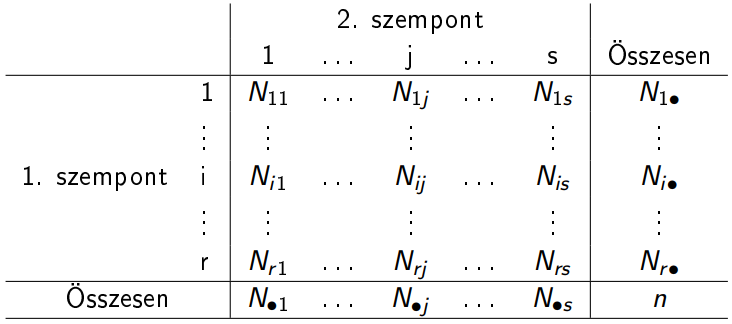
\includegraphics[width=0.7\linewidth]{függetlenségvizsgálat}
\end{figure}

\subsubsection{Függetlenségvizsgálat R-ben}

\begin{outline}
	\1 \texttt{chisq.test(matrix(c(15, 10, 10, 10), ncol=2, byrow=TRUE))}
		\2 Értelmes táblázat/mátrix kezelés: lásd R jegyzet (lejjebb)
\end{outline}

\pagebreak

\subsubsection{Függetlenségvizsgálat R-ben manuálisan}

\begin{verbatim}
rows <- nrow(tablazat); cols <- ncol(tablazat)
probastat <- 0; for (i in 1:rows) for (j in 1:cols) {
  tmp <- sum(tablazat[i,]) * sum(tablazat[, j]) / sum(tablazat)
  probastat <- probastat + (tablazat[i, j] - tmp)^2 / tmp }
pertek <- 1 - pchisq(probastat, (rows - 1) * (cols - 1))
cat('Próbastatisztika:', probastat,
    '\nKritikus érték', qchisq(1 - alpha, (rows - 1) * (cols - 1)),
    '\nP-érték:', pertek,
    '\nDöntés:', if (pertek < alpha) { 'H0 elutasítva' }
    else { 'H0-t nem sikerült elvetni' }, '\n')
\end{verbatim}

\pagebreak

\subsection{Korreláció- és regresszióelemzés}

\subsubsection{Korreláció}

\begin{outline}
	\1 Korreláció: szimmetrikus, két változó lineáris kapcsolatának erőssége
	\1 Értéke: -1 és 1 között, ahol -1 az erős negatív kapcsolat
		\2 Függetlenség esetén az együttható 0 (visszafelé nem igaz)
	\1 Elméleti korrelációs együttható: $R(X,Y) = \frac{cov(X,Y)}{D(X)D(Y)}
	= \frac{E((X-E(X))(Y-E(Y)))}{D(X)D(Y)}$
	\1 Pearson tapasztalati korreláció: $r_{X,Y} =
	\frac{\sum_{1}^{n}(X_i - \overline{X})(Y_i - \overline{Y})}{(n-1 )S_X S_Y}
	= \frac{\sum_{1}^{n}(X_i - \overline{X})(Y_i - \overline{Y})}
	{\sqrt{ \sum (x_i - \overline{X})^2 * \sum (y_i - \overline{Y})^2 }}$
		\2 R-ben: \texttt{cor(x,y)}\\
		vagy \texttt{sum((x-mean(x))*(y-mean(y))) / ((length(x)-1)*sd(x)*sd(y))}
\end{outline}

\begin{figure}[h!]
	\centering
	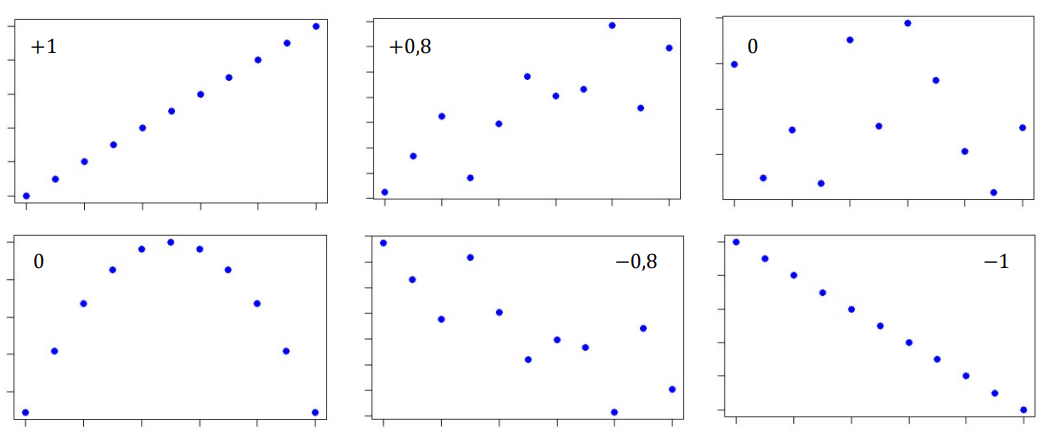
\includegraphics[width=0.7\linewidth]{korreláció}
\end{figure}

\subsubsection{Regresszió}

\begin{outline}
	\1 Regresszió: két vagy több változó között fennálló kapcsolat modellezése
		\2 Egyszerű lineáris regresszió: két változó irányított lineáris kapcsolata
	\1 $y_i = a + bx_i + \epsilon_i$ ahol $y$ függő/eredmény és $x$ magyarázó
		\2 $E(\epsilon)=0$ és $D^2(\epsilon) = \sigma^2 < \infty$ (normál eloszlás)
		\2 $X$ legyen hiba nélküli (vagy elhanyagolható hibájú)
	\1 Bármely jelölésen kalap: konkrét értéket jelent (pl. $\widehat{\epsilon_i} = y_i - \widehat{y_i}$)
	\1 Legkisebb négyzetek módszer: $\min \sum_{i=1}^{n} ( y_i - (a+bx_i) )^2$
\pagebreak
	\1 Reziduális: becsült és valós $y$ függőleges távolsága adott $x$ esetén
	\1 Hiba szórásnégyzet becslés: $\widehat{\sigma}^2 = \frac{\sum (y_i - \widehat{y_i})^2}{n-2}$
	\;\; (residual standard error)
	\1 Determinációs együttható:
		\2 $0 \le R^2 \le 1$, minél nagyobb, annál jobb a modell
		\2 Megadja, hogy $Y$ változásainak hány százalék magyarázza a modell
		\2 Sima: $R^2 = 1 - \frac{\sum(y_i - \widehat{y_i})^2}{\sum(y_i - \overline{y})^2}$
			\3 Nő, ha több magyarázó változót használunk, tehát nem ideális
		\2 Korrigált: $R^2_{adj} = 1 - (1-R^2) \frac{n-1}{n-p}$ ahol $p$ a változók száma (itt: 2)
	\1 R-ben: \texttt{summary(lm(függő $\sim$ magyarázó))} \;\; (két vektor)
		\2 \texttt{Residuals}: kevés adat esetén az értékek, sok esetén összesítés
		\2 \texttt{Intercept} sor: $a$ értéke (függőleges eltolás)
		\2 \texttt{Estimate} oszlop: $a$, $b$ értéke (szorzó)
		\2 \texttt{Pr(>|t|)} oszlop: mennyire fontos ez a változó a modellbenó
			\3 $H_0$: lehetne 0, el lehetne hagyni a változót
			\3 $H_1$: nem 0, azaz fontos a változó
			\3 \texttt{Pr(>|t|)} $< \alpha = 0.05 \implies$ fontos a változó, $H_0$ elvetve
		\2 \texttt{Residual standard error}: reziduális szórás becslése, $\sqrt{\widehat{\sigma}^2}$
		\2 \texttt{Multiple/Adjusted R-squared}: (korrigált) determinációs együttható
	\1 Hasznos R függvények:
		\2 Legyen \texttt{reg <- lm(y $\sim$ x)}
		\2 Ábrázolás: \texttt{plot(x,y); lines(x, reg\$fitted.values)}
		\2 Kiszámolás adott $x$-re: \texttt{reg\$coefficients[1] + adottX * reg\$coefficients[2]}
	\1 Manuális "megoldása" $y=a+bx$-nek
		\2 $\hat{b} = \frac{cov(X,Y)}{D^2(X)}$ \; (R-ben: \texttt{cov(x,y) / sd(x)\^{}2})
		\2 $D^2(\hat{b}) = \frac{\sigma^2}{\sum(x_i - \overline{X})^2}$
		\2 $\hat{a} = EY - \hat{b}EX$ \; (R-ben: \texttt{mean(y) - $\hat{b}$*mean(x)})
		\2 $D^2(\hat{a}) = \sigma^2(\frac{1}{n} + \frac{\overline{X}^2}{\sum(x_i - \overline{X})^2})$
\end{outline}

\pagebreak

\section{Előadás 12: lineáris modell, logisztikus regresszió, vegyes kapcsolat}

\begin{outline}
	\1 TODO 12. előadás
	\1 Remélhetőleg nem lesz benne a ZH-ban: gyakorlaton se néztük
\end{outline}

\pagebreak

% EA - GYAK elválasztó

\section{R jegyzet}

\subsection{Hasznos R függvények}

\begin{outline}
	\1 Indexek, ahol \texttt{TRUE} van: \texttt{which(x == max(x))}
\end{outline}

\subsection{Grafikonok, plot-ok}

\begin{outline}
	\1 \begin{verbatim}plot( c(...) )\end{verbatim}
	\1 \begin{verbatim}plot(x, y, type = "l", ...)\end{verbatim}
	\1 \begin{verbatim}plot(seq(from, to, 0.01), sapply(..., f), ...)\end{verbatim}
	\1 \begin{verbatim}barplot(f(0:100), names.arg=0:100, ...)\end{verbatim}
	\1 \begin{verbatim}boxplot(wt ~ cyl, data = mtcars, ...)\end{verbatim}
		\2 \$out: outlier values
	\1 \begin{verbatim}hist(x, breaks=5)\end{verbatim}
		\2 \$counts: gyakoriságok osztályokban
\end{outline}

\subsection{Matematikai függvények}

\begin{outline}
	\1 sum(x), sort(x), min(x), max(x), round(x, 4)
	\1 Mintaátlag, $\overline{X}$: \texttt{mean(x)}
	\1 Korrigált tapasztalati szórás, $S^*_n$: \texttt{sd(x)}
	\1 Korrigált szórásnégyzet, $(S^*_n)^2$: \texttt{var(x)}
	\1 Tapasztalati k-adik momentum, $m_k$: \verb|mean(x^2)|
	\1 Statisztikák (min, max, átlag, kvartilisek): \texttt{summary(x)}
	\1 Kvartilis: \texttt{quantile(x, probs = c(1/4, 1/2, 3/4), type = 6)}
	\1 Tapasztalati eloszlásfüggvény: \texttt{plot(ecdf(x), ...)}
\end{outline}

\pagebreak

\subsection{Adathalmaz}

\begin{outline}
	\1 $mtcars$ egy adathalmaz, aminek van $cyl$ és $wt$ oszlopa
	\1 \begin{verbatim}subset(mtcars, cyl == 4)$wt\end{verbatim}
	\1 \begin{verbatim}mtcars[mtcars$cyl == 4,]$wt\end{verbatim}
	\1 Érték-gyakoriság táblázat: \texttt{table(vektor)}
		\2 Oszlop, ahol <valami> igaz: \texttt{names(tábla)[tábla==max(tábla)] }
\end{outline}

\subsection{Táblázat, mátrix}

\begin{verbatim}
ido <- matrix(c(15, 10, 5, 10, 10, 20, 5, 20, 5), ncol=3, byrow=TRUE)
colnames(ido) <- c("kevés", "átlagos", "sok")
rownames(ido) <- c("hüvös", "átlagos", "meleg")
ido <- as.table(ido)\end{verbatim}

\end{document}
